\documentclass[a4paper,oneside]{article}

\usepackage[utf8]{inputenc}
\usepackage[T2A]{fontenc}
\usepackage[english,russian]{babel}

\usepackage{amsmath}
\usepackage{mathtools}
\usepackage{amsfonts}
\usepackage{enumitem}
\usepackage{amsthm}
\usepackage{minted}
\setminted{fontsize=\small, breaklines=true, style=emacs, linenos}
\usepackage{graphicx}
\graphicspath{ {./images/} }
\usepackage{float}

\newtheorem{theorem}{Теорема}[subsection]
\newtheorem*{theorem*}{Теорема}

% --- Определение --- %
\theoremstyle{definition}
\newtheorem{definition}{Определение}[subsection]
\newtheorem*{definition*}{Определение}
% ------------------- %

\title{{Теория кодирования и сжатия информации}\\{Лабораторная работа №1}}
\author{Гущин Андрей, 431 группа, 1 подгруппа}
\date{\the\year{} г.}

\begin{document}

\maketitle

\section{Задача}

Разработать программу осуществляющую архивацию и разархивацию текстового файла
используя алгоритм Хаффмана. Программы архивации и разархивации должны быть
представлены отдельно и работать независимо друг от друга. Определить для
данного шифра характеристики 1 (коэффициент сжатия) и 2 (скорость сжатия). К
работе необходимо прикрепить отчет и программный проект.


\section{Алгоритм}

Алгоритм Хаффмана заключается в создании нового кода для каждого встречающегося
в тексте символа на основе частоты встречи этого символа.

Алгоритм состоит из следующих шагов:
\begin{enumerate}
    \item Вычислить частоты всех встретившихся символов;
    \item Построить очередь с приоритетом на основе полученных частот;
    \item Построить дерево с помощью очереди с приоритетом;
    \item На основе дерева вычислить код для каждого символа.
\end{enumerate}


\section{Тестирование}

Для проверки программы были использованы тестовые тексты 1 (рис.
\ref{fig:test_1}) и 6 (рис. \ref{fig:test_6}). Можно заметить,
что после распаковки архива полученный файл совпадает с исходным (проверка
с помощью утилиты diff). Также можно заметить, что для файлов малого размера
архив увеличивает их размер за счёт метаданных.

\begin{figure}[H]
    \centering
    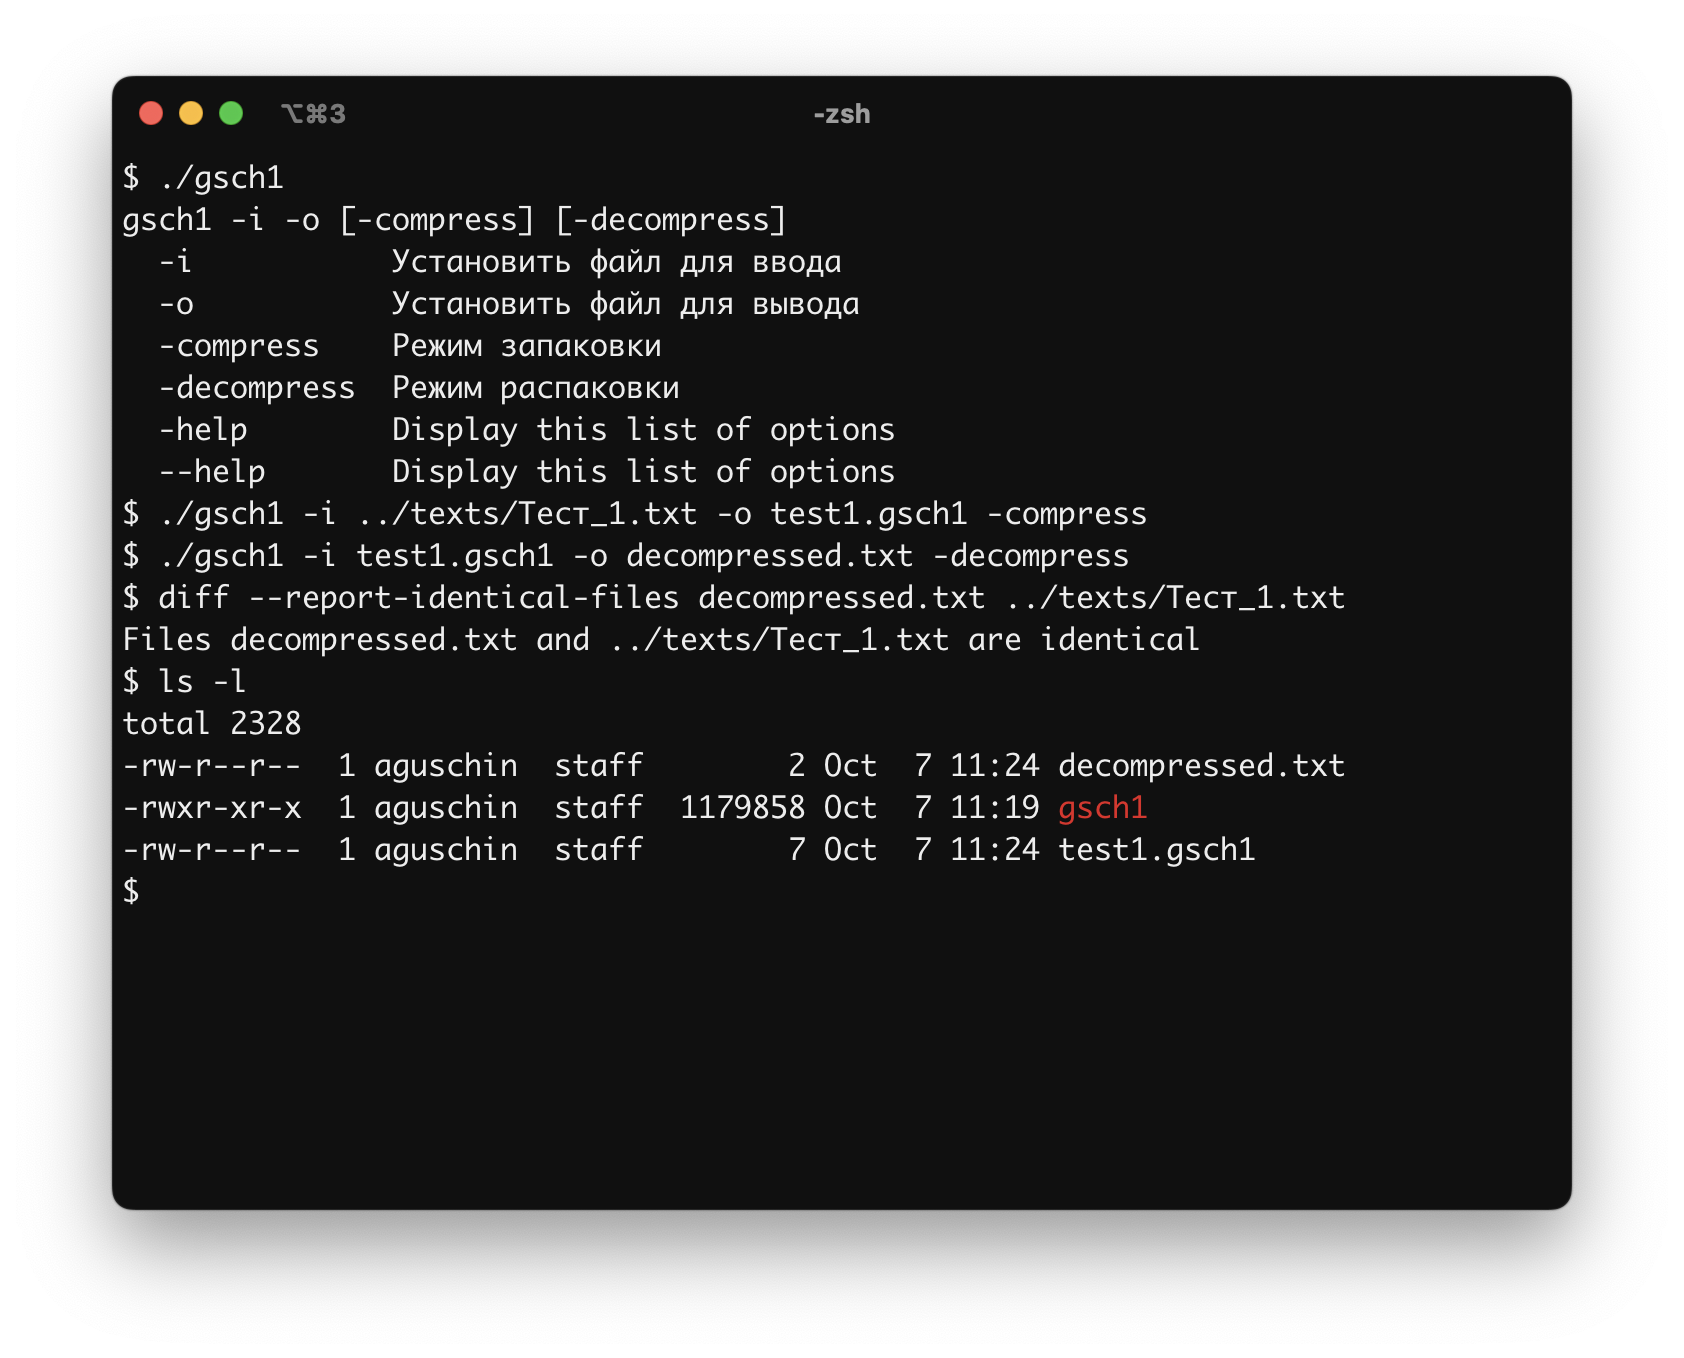
\includegraphics[width=0.9\textwidth]{test1.png}
    \caption{Сжатие текста Тест\_1.txt}
    \label{fig:test_1}
\end{figure}

\begin{figure}[H]
    \centering
    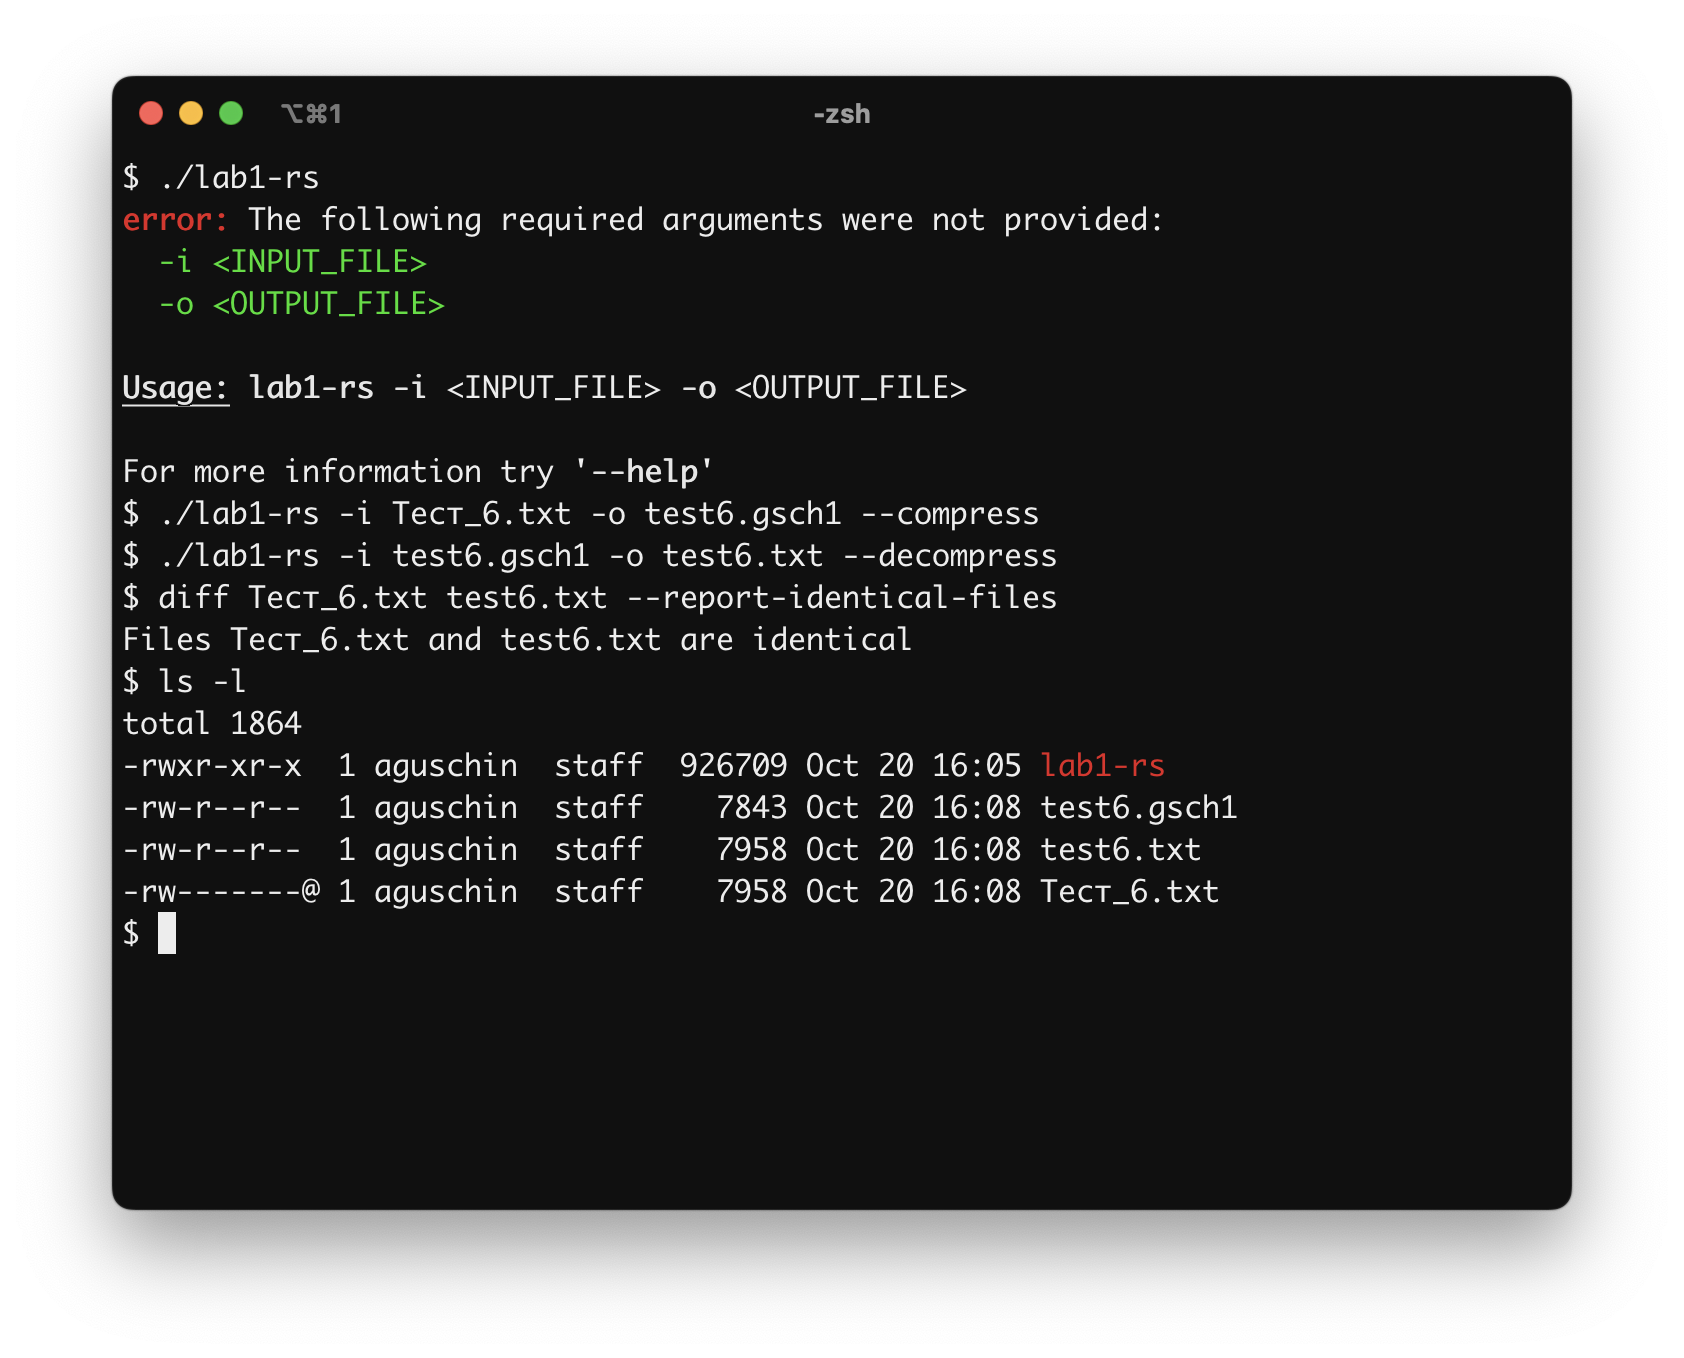
\includegraphics[width=0.9\textwidth]{test6.png}
    \caption{Сжатие текста Тест\_6.txt}
    \label{fig:test_6}
\end{figure}


\section{Вычисленные характеристики}

\subsection{Характеристика 1 (Коэффициент сжатия)}

Результаты применения программы к каждому из тестовых текстовых файлов занесены
в таблицу \ref{tbl:results}. Можно заметить, что в некоторых случаях архивация с
помощью алгоритма Хаффмана является неэффективной.

\begin{table}[H]
    \small
    \centering
    \begin{tabular}{|c|c|c|c|}
        \hline
        Название     & Исходный размер, байт & Сжатый размер, байт & Коэффициент \\ \hline \hline
        Тест\_1.txt  & 2                     & 7                   & 0.28571     \\ \hline
        Тест\_2.txt  & 33                    & 92                  & 0.3587      \\ \hline
        Тест\_3.txt  & 2739                  & 1998                & 1.37087     \\ \hline
        Тест\_4.txt  & 330                   & 48                  & 6.875       \\ \hline
        Тест\_5.txt  & 59                    & 168                 & 0.35119     \\ \hline
        Тест\_6.txt  & 7958                  & 7577                & 1.05028     \\ \hline
        Тест\_7.txt  & 138245                & 134049              & 1.0313      \\ \hline
        Тест\_8.txt  & 574426                & 482613              & 1.19024     \\ \hline
        Тест\_9.txt  & 2752                  & 348                 & 7.90805     \\ \hline
        Тест\_10.txt & 2814                  & 708                 & 3.97458     \\ \hline
    \end{tabular}
    \caption{результаты тестирования}
    \label{tbl:results}
\end{table}

\subsection{Характеристика 2 (Скорость сжатия)}

Для тестирования скорости сжатия использовался произвольный двоичный файл
размера 76450438 байт ($\approx$73 мегабайта). В результате пяти последовательных
запусков, среднее время запаковки файла составило 44.08 секунды, среднее
время распаковки составило 33.42 секунды.

Таким образом, средняя скорость сжатия составила 1.65401 Мбайт в секунду, а
средняя скорость разжатия составила 2.18159 Мбайт в секунду.


\section{Реализация}

Программа реализована на языке программирования OCaml с использованием
исключительно стандартной библиотеки языка. Сборка производится с помощью
программы GNU Make и компиляторов ocamlc и ocamlopt, поставляющихся вместе с
языком.

\subsection{Содержимое файла priority\_queue.ml}
\inputminted{ocaml}{../../lab1/priority_queue.ml}

\subsection{Содержимое файла huffman.mli}
\inputminted{ocaml}{../../lab1/huffman.mli}

\subsection{Содержимое файла huffman.ml}
\inputminted{ocaml}{../../lab1/huffman.ml}

\subsection{Содержимое файла compress.ml}
\inputminted{ocaml}{../../lab1/compress.ml}

\subsection{Содержимое файла Makefile}
\inputminted{ocaml}{../../lab1/Makefile}


\end{document}
